\documentclass[conference]{report}
\usepackage{graphicx}
\usepackage{hyperref}
\usepackage{mathtools}
\usepackage{amsmath}
\usepackage{amssymb}
\usepackage{bbm, dsfont}
\usepackage{centernot}
\begin{document}

\def\T{\textbf{T}}
\def\F{\textbf{F}}
\def\NOT{\texttt{NOT}}
\def\AND{\texttt{AND}}
\def\OR{\texttt{OR}}
\def\XOR{\texttt{XOR}}
\def\R{\mathbb{R}}
\def\B{\mathbb{B}}
\def\N{\mathbb{N}}

\def\custop#1{{\mspace{4mu}#1\mspace{4mu}}}
\def\concat{\custop{@}}

\title{\LARGE Designing Interpretable Chess Engines Using Logical Neural Networks}

\maketitle
\thispagestyle{plain}
\pagestyle{plain}

\begin{abstract}
The problem of interpretability in DNNs is classically a hard one, as the parameterisation of network layers is hard to intuit. This paper uses findings in Logical Neural Network architectures to construct an interpretable model for use cases which are easily modelled by logical statements, and applies this architecture to the problem of learning Chess.  
\end{abstract}

\tableofcontents

\pagebreak

\chapter{Interpretability}

\section{Introduction}

Research into problems in Machine Learning in recent years has focused largely into using Neural Network (NN) models to solve increasingly broad categories of problems. NNs, much like many other models, define a hypothesis class of functions which differ only in their parameterisation, and uses Stochastic Gradient Descent (SGD) or some descendant thereof, to optimise said parameters given a loss function. Classical Multi-Layer Perceptrons (MLPs) consist of a series of linear layers separated by some non-linearity, (e.g. ReLU, Sigmoid functions). Given certain conditions, it is known that MLPs can learn any continuous function to arbitrary precision, by the Universal Approximation Theorem (UAT). The effectiveness of SGD methods allows us to learn arbitrary functions tractably given sufficient data, which has resulted in a widespread adoption of the architecture in practical settings.

A common criticism of NNs, however, is that they are considered ``black box" functions. NNs are difficult to interpret, making it even more difficult to diagnose issues that may arise in production. A particular node in the network may be considered as capturing a single ``concept", which can further be used to determine the presence of other concepts. It is difficult, however, to interpret how these concepts are generated - taking linear combinations of features and then applying a non-linear map to the result is not a terribly human line of thinking when it comes to pattern recognition. In this way, when comparing NNs to real-world neural processes, the description of NNs capturing general human intuition, rather than any kind of conscious reasoning, is most apt.

The ``black box" nature of NNs has resulted in a hesitancy for it's adoption in particular settings, most notably in the medical industry, where even small risks of misdiagnosis cannot be tolerated. One would assume that an architecture that is so widely used in so many sensitive settings should be easily examinable, but this isn't that case.

From this, the notion of ``interpretability" is often discussed when developing or analysing novel neural architectures (\cite{interpretbook}, \cite{gradientattribute}, \cite{interpretdeepmodels}). An ideal interpretable model would allow the user to know precisely what the model is achieving by arriving at a particular optimal parameterisation. Interpretability is not a quantifiable metric - the user may gain an understanding through a mixture of the learnt parameters and an existing intuition over the architecture itself. This allows for a wide breadth in methods which may be used to gain an understanding of a model, and also hopefully the underlying problem.

\section{Interpretation Methods}

There are many ways we may attempt to approach the problem of interpretability. Commonly used methods take arbitrary NN architectures, and attempt to gauge how relevant a particular feature of a given input is in the overall output of the model. These are known as \textit{Variable Importance Measures} (VIMs). Gradient-based attribution methods \cite{gradientattribute} are the classical example, where the gradient of the model with respect to its input features are used as the measure of feature importance. This makes intuitive sense, as if the output of the model is subject to large changes with small deviations in an input feature, it must naturally be fairly important. The most commonly seen setting for these methods is in image classification, where the importance of a particular pixel measures how much of an influence said pixel has on determining the category of an image. Plotting the importance of all the pixels hopefully shows the user precisely which portions of the image contain the relevant object to classification. E.g., distinguishing between cats and dogs would largely rely on examining particular features of the face shape, so one would expect these features to be the most important by this metric.

These methods are very versatile, as they are \textit{model-agnostic}. There are many flaws, however - what if the classification of an image relies on a combination of features, rather than just a single one? We can capture this notion by instead using VIMs over all nodes in the network, i.e. the input layers and all hidden layers, but we run into the same problem - if we determine that a node in a hidden layer is important, how do we begin to understand what this node is doing? This method captures relevance, but does not capture what concepts these features may represent - we can leave this again up to the intuition of the user, or we can apply VIMs recursively between the input features and the hidden feature. This eventually becomes somewhat unwieldy. 

Another issue is that VIMs are \textit{local} interpretation methods, as they do not describe the model as a whole - only the model given a set input. This does not give us a good understanding as to why the model's solution to a problem is best.

A solution to the problem of not capturing feature relationships is in developing \textit{model-specific} methods of interpretability. We can design an architecture which allows for novel ways of visualising model behaviour, often by restricting the expressiveness of the model in a manner which allows the remaining hypothesis class to be easily distinguishable. 

One example of such an architecture are Neural Additive Models (NAMs) \cite{neuraladditive}. Neural Additive Models are a generalisation of General Additive Models (GAMs) in that they are fully described by the equation
$$M(\vx) = \sigma\left(\sum_i M_i(x_i)\right)$$

Where the $M_i:\R \mapsto \R$ represent univariate NNs, and $\sigma$ is the \textit{link function}.

In backpropagation, we learn the parameters of each subnetwork $M_i$ simultaneously. Given that each subnetwork is a map $\R \to \R$, we can capture the behaviour of the model not only locally through VIMs, but globally, as we can easily plot the value of $M_i$ over the entire domain. Simply observing this graph allows the user to speculate as to what the model has learnt.

This model, while very interpretable, is not very expressive - we cannot capture any relationships between variables that aren't described by the link function $\sigma$, as is the nature of GAMs. This is the very problem we intended to solve by discussing NAMs - we want to be able to capture not only the relevance of input features, but of learnt concepts over those features.

Again, new model architectures have been introduced to resolve this. The aptly named Explainable Neural Network (xNN) \cite{xnn} is an architecture which extends NAMs with a single linear ``projection layer". These are equivalent to learning a GAM over \textit{linear combinations} of input features. They are therefore fully described by the equations
$$
\begin{aligned}
\va &= \vW\vx + \vb\\
M(\vx) &= \sigma\left(\sum_i M_i(a_i)\right)
\end{aligned}
$$

Where $\vW, \vb$ are learnable parameters as standard. We can interpret this model very similarly, by again plotting the univariate subnetworks $M_i$, and simply interpreting what a concept $a_i$ represents by directly observing the linear combination. The UAT tells us that this single added layer is enough to model any function to an arbitrary precision, but in practice this hidden layer would need to be quite wide for anything other than the most trivial problems, and the features introduced in a large hidden layer may not be terribly intuitive to understand, and may even introduce a large bias.

We could extend this further, by adding more perceptron layers to capture more complicated relations between input features, but this naturally comes at the expense of interpretability. An ideal solution to this problem would allow for the model to be extended with more layers without sacrifice.

This motivates a new architecture for layers in our NN, as perceptron layers can be considered the main obstruction to interpreting our models.


\chapter{Logical Neural Networks}

\section{Introduction}

We will discuss an NN architecture which attempts to learn boolean functions, instead of real functions. The restricted nature of boolean functions, and their use as a mathematical description of logic, allows a intuitive way of representating causation (e.g., if for some object $x$). The models that are created to solve such a problem are known as \textit{Logical Neural Networks}\footnote{also \textit{Neural Logic Networks, Logic Tensor Networks}} (LNNs)\footnote{also NLNs, LTNs}. The subfield of ML concerned with learning solutions to logical problems with gradient-descent based methods is called \textit{Neurosymbolic Machine Learning}.

The goal of the LNNs we discuss here will be to learn the optimal assignments for boolean variables within a statement described by the language of first order logic. This parallels the goal of MLPs to learn the optimal assignments for real variables within linear layers. LNNs achieve this through continuous optimisation using the standard approach of applying SGD methods with backpropagation. 

It is interesting to note that the most widely researched approaches within the field of Artificial Intelligence (AI) until the 1990s were symbolic-based methods. There are many well studied algorithms that, given a set of logical predicates known to be true, attempt to capture the nature of the wider system in a single (ideally simple!) logical statement. These algorithms are known as Inductive Logic Programming (ILP) systems \cite{ilp}. While very useful, they were found to be computationally intractible for more complex problems, notably those in Computer Vision and Natural Language Processing. Famously, Hubert Dreyfus predicted that symbolic methods were inherently incapable of fully capturing the complexity of such problems \cite{symbolicaibad}, stating that these relied primarily on unconscious processes rather than conscious symbolic manipulations. It seems most apt, therefore, to understand the rise of Deep Learning methods in the new millenium as reliant on capturing such ``unconscious'' processes.

The aim of neurosymbolic methods are thus to be able to capture the expressiveness of Deep Learning methods, without sacrificing the interpretability afforded by understanding the model in terms of symbolic manipulations. This is a difficult task! 

\section{Real Logic}

We run into the important issue of $\{\T, \F\}$, the space of boolean values, not being continuous. One way of solving this issue is by extending the domain of possible logical assignments from $\{0,1\}$, as above, to the closed interval $[0,1]$. This is referred to as both \textit{real logic}, (as in \cite{ltn2016}, \cite{analyzefuzzy}, and much of the literature focusing on differentiable applications), and \textit{fuzzy logic} (as in most foundational literature, namely \cite{fuzzysetbook}, \cite{fuzzylogicbook}, \cite{fuzzymetabook}). Using the name ``fuzzy logic'' emphasises the importance of properties which are not relevant to the neurosymbolic architecture we will be discussing here, so we will not be using the term widely, but many of the following constructions are drawn from literature on fuzzy logic. We will discuss approaches in extending important logical operators ($\OR$, $\AND$, $\NOT$, ...) to this new boolean space, and ways we may begin to use it to learn in an interpretable way. 

To fully define a ``real logic", that is, an extension of classical logic to the space $[0,1]$, we want to define all the operators in a manner that, ideally, preserves many of the useful properties we see in the classical definition. At the very least, we want the values over the restricted domain $\{0,1\}$ to be the same as in classical logic.

It is well known that given a finite number of variables $\{x_i\mid i \in 1 , \dots, N \}$, all boolean functions (that is, functions $\phi : \{\T,\F\}^N \rightarrow \{\T,\F\}$) can be expressed in terms of the operators $\lnot$ and $\land$. Explicitly,
$$
\begin{aligned}
    a \lor b &= \lnot (\lnot a \land \lnot b) \\
    a \limply b &= \lnot (a \land \lnot b) \\
    a \lxor b &= \lnot(a \land \lnot b) \land \lnot(\lnot a \land b) \\
    a \lxnor b &= \lnot(a \land b) \land \lnot(\lnot a \land \lnot b) \\
    \forall x, \phi(x) &= \phi(x_1) \land \dots \land \phi(x_N) \\
    \exists x, \phi(x) &= \lnot(\lnot \phi(x_1) \land \dots \land \lnot \phi(x_N)) \\ 
\end{aligned}
$$

If we can extend the operators $\land$ and $\neg$ to the full domain $[0,1]$, we can therefore do so for all the above operators also. For the remainder of this section, we will specify that $\T \coloneqq 1$, and $\F \coloneqq 0$, though we will later see examples where this is not the case.

\subsection{Real Conjunction and Negation}

We will take a set of properties that apply to classical conjunction $\land$ and require that the extension $\land : [0,1]^2 \to [0,1]$ has them also. The properties are;

$$
\begin{aligned}
\text{(Associativity)}&\ (a \land b) \land c = a \land (b \land c) \\
\text{(Commutativity)}&\ a \land b = b \land a \\
\text{(Monotonicity)}&\ a \leq b, c \leq d \implies a \land c \leq b \land d \\
\text{(Identity)}&\ \forall a \in [0,1], a \land 1 = a
\end{aligned}
$$

The above are known as the \textit{T-norm axioms} \cite{tnorms}. Note that they are a strict subset of the axioms required for $([0,1], \land, \lor)$ to be a boolean algebra, namely we are missing distributivity and idempotence. In fact, it is possible to construct a real logic that preserves these properties also, but there is precisely one such logic, and as we will see, it has flaws that make it less than ideal for gradient descent. The above axioms are, however, enough for $\land$ to have the correct output for the restricted domain $\{0,1\}$. 

We can likewise define negation simply by $\lnot : x \mapsto 1 - x$. In the fuzzy logic literature, this is known as \textit{strong negation}, as there is an alternate formulation of negation that captures the intention of fuzzy logic more effectively.

It can be shown that the axioms as we have defined them allow for an infinite family of possible real logics. Some examples are given below;

\begin{center}
\begin{tabular}{ c | c c }
    Logic & $\forall$ & $\exists$ \\    
    \hline
    Minimum 
    & $\min\{ x_1, \dots, x_N \}$ 
    & $\max\{ x_1, \dots, x_N \}$ \\ 
    Product 
    & $\prod_ix_i$
    & $1 - \prod_{i}(1-x_i)$ \\
    Łukasiewicz
    & $\max\{\sum_ix_i - N + 1, 0\}$ 
    & $\min\{\sum_ix_i, 1\}$ \\
    Schweizer-Sklar
    & $\max\{\sum_ix^p_i - N + 1, 0\}^\frac{1}{p}$ 
    & $\min\{N-\sum_i(1-x_i)^p, 1\}^\frac{1}{p}$ \\
    Yager
    & $\max\{1 - (\sum_i(1-x_i)^p)^\frac{1}{p}, 0\}$ 
    & $\min\{(\sum_ix^p_i)^\frac{1}{p}$, 1\} \\
\end{tabular}
\end{center}

The examples are expressed as conjunctions of $N$ variables, not just 2. $p$ in the table above is a hyperparameter. Figures \ref{fig:conjplots} shows more visually how some of these logics behave.

\begin{figure}[h]
    \centering
    \begin{subfigure}[b]{0.2\textwidth}
        \centering
        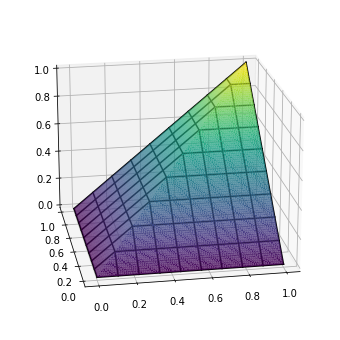
\includegraphics[width=\textwidth]{imgs/fuzzy_min_and.png}
        \caption{Minimum}
        \label{fig:minconj}
    \end{subfigure}
    \begin{subfigure}[b]{0.2\textwidth}
        \centering
        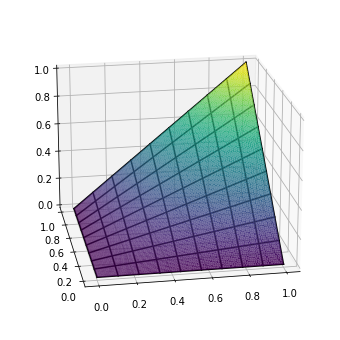
\includegraphics[width=\textwidth]{imgs/fuzzy_prod_and.png}
        \caption{Product}
        \label{fig:prodconj}
    \end{subfigure}
    \begin{subfigure}[b]{0.2\textwidth}
        \centering
        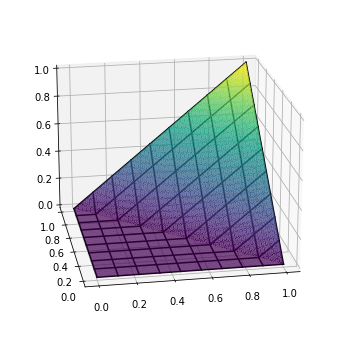
\includegraphics[width=\textwidth]{imgs/fuzzy_luk_and.png}
        \caption{Łukasiewicz}
        \label{fig:lukconj}
    \end{subfigure}
    \begin{subfigure}[b]{0.2\textwidth}
        \centering
        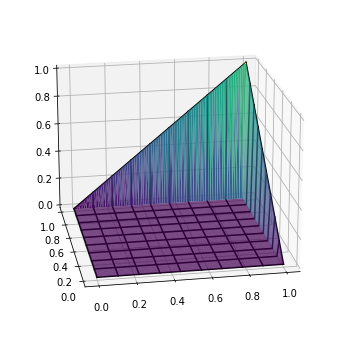
\includegraphics[width=\textwidth]{imgs/fuzzy_dra_and.png}
        \caption{Drastic}
        \label{fig:draconj}
    \end{subfigure}
       \caption{Conjunction over various fuzzy logics. Note how pointwise gradients differ.}
       \label{fig:conjplots}
\end{figure}

\section{General Architectures}
\label{section:fuzzyloss}

Now that we have explicit definitions for boolean-like algebras in the domain $[0,1]$, we can begin to formulate how we may learn in this setting.

We first need to consider what problems we may want to solve. A basic problem is that of \textit{satisfiability}, i.e., given a boolean function $\phi : \{0,1\}^K \rightarrow \{0,1\}$ which can be expressed in first-order logic, is there some element $\vx \in \{0,1\}^K$ such that $\phi(\vx) = 1$? If so, we want to find an example of said $\vx$.

We can consider this as a continuous optimisation problem with $\vx$ as a parameter. We can extend $\phi$ to the real domain $[0,1]$ by extending each operator in $\phi$ when expressed in the language of first-order logic. Then, by performing SGD as normal, we aim to minimise the loss function $\ell(\vx) = \lnot\phi(\vx)$.

To match the power of classical MLPs, we also want to be able to learn optimal \textit{functions} $\phi$. Suppose we have a dataset $\{(\vx_i, y_i)\}_{i=1}^N$ where $\forall i, \phi(\vx_i) = y_i$ for some formula $\phi : \{0,1\}^K  \rightarrow \{0,1\}$ which need not have a known representation in classical first-order logic. Further suppose we have a function $\psi : \{0,1\}^{K+P} \rightarrow \{0,1\}$ expressed in first-order logic such that for some $\vw \in \{0,1\}^P$, $\phi(\vx) = \psi(\vx, \vw)$. We consider $\vw$ a parameter here, to be optimised. We could use a variety of losses, in the following we examine $\ell(\vx, y; \vw) = (y \lxor \psi(\vx, \vw))^a$, for some exponent $a \in [1,\infty)$ (as $\bbE_{\vx}[\ell(\vx, \phi(\vx); \vw)] = 0 \iff \psi(\vx, \vw) = \phi(\vx)$), which we refer to as $\XOR$ loss, and binary cross-entropy, as is done in \cite{embeddedlogicreg}. 

It is very feasible to find expressive enough $\psi$, as it can be shown that every boolean function $\phi$ can be expressed in a number of standard forms - Disjunctive Normal Form (DNF), and Conjunctive Normal Form (CNF), being two notable ones. To fit these two representations into the framework we have described, we need to be able to express how every variable $x_i$ is represented in each normal form by appending appropriate parameter variables $w_i$.

In DNF, $\phi$ is expressed as a disjunction of conjunctions, with each conjunction described by a subset of input variables $\subseteq \{x_1,\dots,x_K\}$, each variable being optionally negated. We can capture membership by boolean variables $m_i \in \{0,1\}$, and negation by $s_i \in \{0,1\}$. This allows us to represent a formula in DNF by

$$
\begin{aligned}
\phi(\vx) &= \exists j,\ 1 \leq j \leq W,\ \phi_j(\vx) \\
\text{where } \phi_j(\vx) &= \forall i,\ m_{ij} \limply (x_i \lxor s_{ij})
\end{aligned}
$$

for some assignment to the $M = (m_{ij}), S = (s_{ij})$. A similar form for CNF is,

$$
\begin{aligned}
\phi(\vx) &= \forall j,\ 1 \leq j \leq W,\ \phi_j(\vx) \\
\text{where } \phi_j(\vx) &= \exists i,\ m_{ij} \land (x_i \lxor s_{ij})
\end{aligned}
$$

In both cases, we can construct a function $\psi$ with $M$ and $S$ as parameters, and optimise over these parameters as before. Here $W \in\bbN$ is a hyperparameter which specifies the number of conjunctions (or disjunctions) in the function family $\psi$. Naturally, the larger $W$ is, the more expressive $\psi$ can be, and we know that $W = 2^K$ is enough to capture all possible functions $\phi$. This very closely parallels the Universal Approximation Theorem (UAT) of MLPs with one hidden layer. It also very closely mirrors the concept of ``reducing induction to satisfiability'' seen in many ILP systems \cite{diffilp}.

\section{Analysis of a Toy Problem}

The framework we have given is very general, and does not specify what real logic we are required to use. Indeed it does not even require that every operation need be from the same logic, only that they are correct on classical boolean values $0,1$. It is valuable, therefore, to compare each logic and analyse which logics are useful for which learning tasks.

In \cite{analyzefuzzy}, the problem of satisfiability over $\phi(a,b,c) = (a \land b) \lor (c \land \lnot a)$ is considered. We compare the convergence of $a, b, c$ \footnote{In practice, we actually consider satisfiability over parameters $a, b, c \in \bbR$ mapped into $[0,1]$ with a sigmoid function, as we want to converge to parameters in the appropriate bounds.} over each logic, given randomly initialised starting parameters.

Figure \ref{fig:toyconv} show convergence of the output of $\phi$ for 1000 uniformly sampled random initialisations of the parameters $a, b, c$ in the interval $(0,1)$, using Adam optimisation \cite{adam} with a learning rate of $10^{-1}$. Convergence to $1$ represents finding a satisfying assignment, whereas anything else represents a failure to do so.

\begin{figure}[h]
    \centering
    \begin{subfigure}[b]{0.45\textwidth}
        \centering
        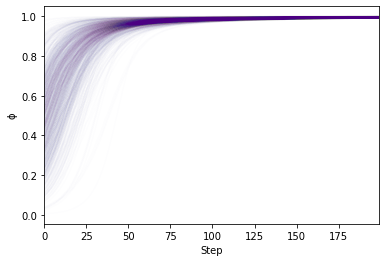
\includegraphics[width=\textwidth]{imgs/toyconv_min.png}
        \caption{Minimum}
        \label{fig:toymin}
    \end{subfigure}
    \begin{subfigure}[b]{0.45\textwidth}
        \centering
        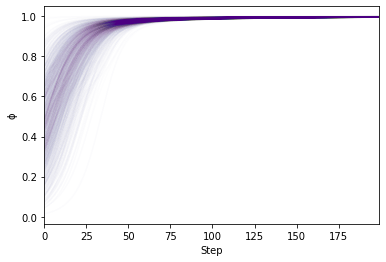
\includegraphics[width=\textwidth]{imgs/toyconv_prod.png}
        \caption{Product}
        \label{fig:toyprod}
    \end{subfigure}
    \begin{subfigure}[b]{0.45\textwidth}
        \centering
        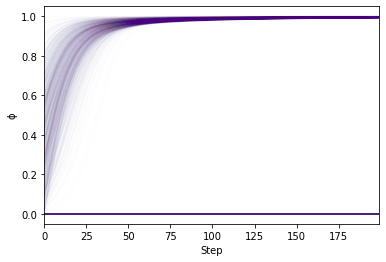
\includegraphics[width=\textwidth]{imgs/toyconv_luk.png}
        \caption{Łukasiewicz}
        \label{fig:toyluk}
    \end{subfigure}
    \begin{subfigure}[b]{0.45\textwidth}
        \centering
        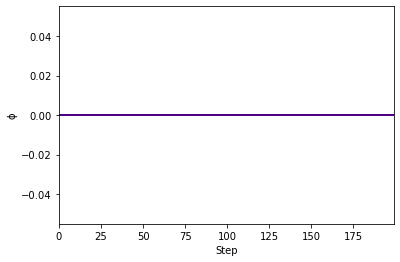
\includegraphics[width=\textwidth]{imgs/toyconv_dra.png}
        \caption{Drastic}
        \label{fig:toydra}
    \end{subfigure}
       \caption{Convergence of toy problem $\phi(a,b,c) = (a \land b) \lor (c \land \lnot a)$ for various fuzzy logics.}
       \label{fig:toyconv}
\end{figure}

We see that the choice of logic has a profound impact on the convergence. Minimum and Product logic both reliably find a satisfying assignment of $\phi$ regardless of initialisation. Łukasiewicz logic finds a satisfying assignment in many instances, but very often fails to optimise at all. Drastic logic (somewhat obviously) never finds a satisfying assignment, regardless of initialisation.

\subsection{Vanishing Gradients}
\label{section:tnormzerograd}

The tests show that a majority of gradient samples for Łukasiewicz logic are precisely $0$. By inspection of Figure \ref{fig:lukconj}, we can see that there are large regions (i.e. regions of non-zero measure) where the function evaluates only to $0$. It is natural that some observations would not allow us to make any meaningful inferences about the optimal values of each variable, especially in cases where the proportion of satisfying inputs is incredibly small. We observe however, that different choices of logic result in different proportions of vanishing gradient observations.

To explain this, we must discuss the nature of conjunction in each logic. In Łukasiewicz logic, for $a, b \in [0,1]$ such that $a + b - 1 < 0$, the gradient of binary conjunction $\land$ is precisely $0$. This means that a full $\frac{1}{2}$ of all possible input arguments (uniformly distributed) give no meaningful inference. Aggregating over $K$ variables, this generalises to a proportion of $1 - \frac{1}{K!}$ inputs having vanishing gradients, which is very obviously not ideal.

Therefore, in this framework, we prefer to use logics such that $\land$ has non-vanishing gradient almost everywhere - these logics are known as \textit{strict}. Minimum and Product logics satisfy this condition, along with certain parameterisations of the Schweizer–Sklar and Yager logics.

\section{Learning Functions}

There are many well known algorithms for efficiently learning classical boolean functions $\phi : \{0,1\}^K \to \{0,1\}$ given prior knowledge of $\phi$ restricting it to a given family. Such algorithms often make logical inferences to determine the proper state of boolean parameters $\vw$, with complexity guarantees that can be described within the Probably Approximately Correct (PAC) learning framework \cite{clt}. We will compare such algorithms to their equivalents in differentiable real logic, and hope for results as good, if not better, given an ideal optimisation regime. 

Generalising these methods to real logic would have considerable benefits. For one, given gradient descent is by nature stochastic and (aside from current parameterisation) stateless, these methods would be inherently robust to noisy data and distribution shift in the learning dataset. A possible drawback is that correctness may only be guaranteed for data drawn similarly to the training dataset, introducing a potentially unavoidable bias.

In each test, we also train a traditional MLP model on the same data. Prior to the test, we could make the assumption that the inductive bias introduced by our model could improve the rate of convergence, but an equally convincing sentiment is that this same bias could be too restrictive on the learning process, slowing down convergence.

\subsection{Learning Conjunctions}

The problem of learning conjunctions is a classical one in Computational Learning Theory (CLT). It is well known that determining conjunctions can be done PAC-efficiently \cite{clt} and is robust to noisy data \cite{noisyclt}. The goal of this comparison, therefore, is simply to prove the viability of real logic for this application.

The classical algorithm relies on one important observation. Suppose $\phi$ is a conjunction, that is - it is a function of the form 
$$\phi(x_1, \dots, x_K) = y_1 \land \dots \land y_N$$

for $y_i \in \{x_1, \dots, x_K, \lnot x_1, \dots, \lnot x_K\}$. If for some $j$, we have $\lnot x_j$ but $\phi$ returns true, then $x_j$ is not one of the terms $y_i$. Similarly $x_j \land \phi$ implies $\lnot x_j$ is not one of the terms. If we begin with $\phi$ a conjunction over all possible such terms, and remove terms where possible, we are eventually left only with the terms actually present in the conjunction.

As discussed previously, we can model the same thing in real logic by introducing weight and sign parameters $\vm$ and $\vs$, 
$$\psi(\vx; \vm, \vs) = \forall i,\ 1 \leq i \leq K,\ m_i \limply (x_i \lxor s_i)$$

and optimising $\vm$ and $\vs$. In the following, for initial simplicity, we set $\vs = 0$ (i.e. we assume no signs $\lnot$.) 

We aim to learn conjunctions by randomly initialising values $\vm$, before minimising for some loss function, such as those given in Section \ref{section:fuzzyloss}. Data pairs are generated by randomly sampling bits $\{0,1\}^D$, and mapping them through a predefined goal conjunction with $N$ terms. We vary many aspects of this model, including conjunction size $D$, number of present terms $N$, choice of fuzzy logic, optimiser, learning rate and loss exponent $a$.

Some results using this architecture are not promising. Figure \ref{fig:conjconvnokeepn} shows convergence of the average distance of a parameter from it's optimal (i.e. correct) value, with the $\XOR$ loss $\ell(\vx, y; \vw) = (\psi(\vx;\vw) \lxor y)^a$ using an Adam optimiser with a learning rate of $10^{-2}$, when learning unsigned conjunctions in the Product logic. Each test is run several times, with the convergence of each run plotted on the graph. Both training and test data are uniformly sampled random bits $\{0,1\}^D$, with each epoch representing 10,000 such samples. We see that for low dimensionality, convergence is quite fast, whereas minimal changes occur with dimensionality any higher than 100. This is of course an issue.

\begin{figure}[h]
    \centering
    \begin{subfigure}[b]{0.48\textwidth}
        \centering
        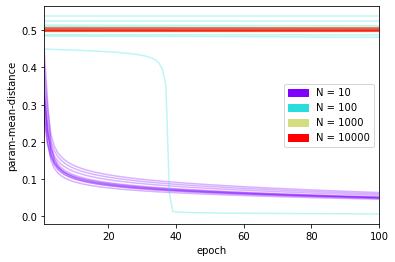
\includegraphics[width=\textwidth]{imgs/conj-pmd-prod-nokeepn-1t.png}
        \caption{1-term conjunction}
        \label{fig:conjconvnokeepn1}
    \end{subfigure}
    \begin{subfigure}[b]{0.48\textwidth}
        \centering
        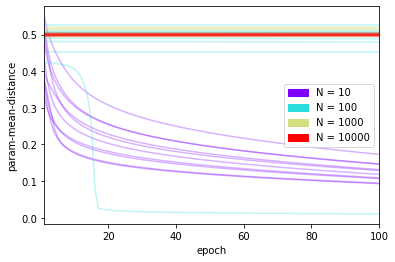
\includegraphics[width=\textwidth]{imgs/conj-pmd-prod-nokeepn-5t.png}
        \caption{5-term conjunction}
        \label{fig:conjconvnokeepn5}
    \end{subfigure}
       \caption{Convergence of mean distance from optimal parameters when learning conjunctions in the Product logic. Each test is run 10 times, with $\XOR$ loss, using exponent $a=10$.}
       \label{fig:conjconvnokeepn}
\end{figure}

We see better results when using binary cross-entropy. Figure \ref{fig:conjconvnokeepnbce} displays the results from the same test, with differing loss function. We see that dimensionality $D=100$ now can be learnt, but we still cannot go much higher.

\begin{figure}[h]
    \centering
    \begin{subfigure}[b]{0.48\textwidth}
        \centering
        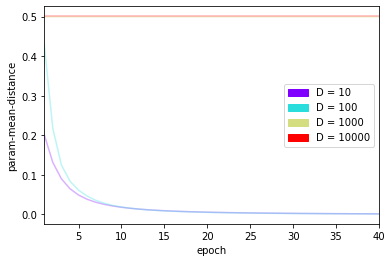
\includegraphics[width=\textwidth]{imgs/conj-pmd-prod-nokeepn-1t-bce.png}
        \caption{1-term conjunction}
        \label{fig:conjconvnokeepn1bce}
    \end{subfigure}
    \begin{subfigure}[b]{0.48\textwidth}
        \centering
        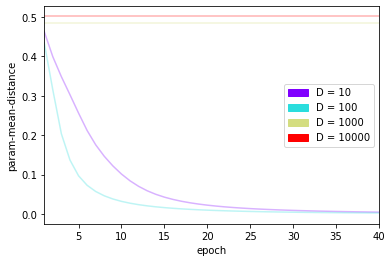
\includegraphics[width=\textwidth]{imgs/conj-pmd-prod-nokeepn-5t-bce.png}
        \caption{5-term conjunction}
        \label{fig:conjconvnokeepn5bce}
    \end{subfigure}
       \caption{Convergence of mean distance from optimal parameters when learning conjunctions in the Product logic, with exponent binary cross-entropy loss.}
       \label{fig:conjconvnokeepnbce}
\end{figure}

\subsection{Vanishing Gradients in Strict Logics}
\label{section:prodvanishgradient}

To determine why this happens, we need only observe the induced gradient of the network. It is well known that a large family of T-norms can be constructed using what is known as an \textit{additive generator}, that is, a function $f$ associated with a given logic, such that $a \land b = f^{-1}(\min\{f(a) + f(b),f(0)\})$. This definition allows us to also say $\forall i, x_i = f^{-1}(\min\{\sum_i f(x_i),f(0)\})$. Some additive generators have $f(x) \rightarrow \infty$ as $x \rightarrow 0$, and in these cases $a \land b = f^{-1}(f(a) + f(b))$ for $a, b \neq 0$.

Suppose $\sum_i f(x_i) \leq f(0)$ (which is trivially satisfied if $\lim_{x\rightarrow 0}f(x) = \infty$). Then;

$$
\begin{aligned}
\forall i, x_i 
&= f^{-1}(\sum_i f(x_i)) \text{, so} \\
\frac{\partial}{\partial x_j} \forall i, x_i 
&= \frac{
f'(x_j)
}{
f'(f^{-1}(\sum_i f(x_i)))
} \\
&= \frac{
f'(x_j)
}{
f'(\forall i, x_i )
}
\end{aligned}
$$

Some examples of additive generators, as well as explicit values for the derivative above, are given in the following table. Note that if $\sum_i f(x_i) > f(0)$, all gradients are vanishing.

\begin{center}
    \begin{tabular}{ c | c c }
        Logic & $f(x)$ & $\frac{\partial}{\partial x_j} \forall i, x_i$ \\    
        \hline
        Product 
        & $-\log x$
        & $\prod_{i \neq j} x_i$ \\
        Łukasiewicz
        & $1 - x$ 
        & $1$ \\
        Schweizer-Sklar
        & $\frac{1-x^p}{p}$ 
        & $\left(\frac{x_j}{\forall i, x_i}\right)^{p-1}$ \\
        Yager
        & $(1-x)^p$ 
        & $\left(\frac{1-x_j}{1-\forall i, x_i}\right)^{p-1}$ \\
    \end{tabular}
\end{center}

The Minimum logic has no additive generator. From the table, the influence of dimensionality now becomes apparent. 

Suppose each aggregate conjunction $\forall i, x_i$ is over $D$ variables. In the product logic, if the $x_i$ are independently uniformly distributed in $[0,1]$, $\bbE\left[\frac{\partial}{\partial x_j} \forall i, x_i\right] = \bbE\left[\prod_{i \neq j} x_i \right] = 2^{D-1}$. Thus the total derivative $\nabla_\forall$ has expected magnitude $\bbE\left[\lVert \nabla_\forall \rVert_2\right] \leq \bbE\left[\sum_j \frac{\partial}{\partial x_j} \forall i, x_i \right] = D2^{D-1}$. With high dimensionality $D$, the gradients quickly degrade.

Other T-norms do not suffer this same issue. For example, Łukasiewicz logic has a gradient of $1$ in every dimension when the function is non-vanishing, however we have shown previously in Section \ref{section:tnormzerograd} that the proportion of vanishing inputs is it's own curse of dimensionality, as it is not strict. Minimum logic has constant $\lVert \nabla_\forall \rVert_2 = 1$, however we will see later that there are still issues with optimisation. In Appendix \ref{section:ssbounds}, we show that for Schweizer-Sklar logic with parameter $p$, the magnitude of $\nabla_\forall$ is lower bounded by $D^{\frac{1}{p}-\frac{1}{2}}$. In this section, we use $p = -2$, thus making the lower bound $D^{-1} \leq \lVert \nabla_\forall \rVert_2$, which is a vast improvement on an upper bound of $D2^{-D}$ seen in the Product logic. Empirical confirmations are given in Figures \ref{fig:conjgrad10100} and \ref{fig:conjgrad10ss100} in the Appendix.

This can also explain why binary cross-entropy performs better than $\XOR$ loss in this domain. With this loss, outputs are mapped through a $\log$ function. If we consider the Product logic, this is equivalent to interpreting conjunctions as a log summation $\sum_i\log x_i$, which means the values of each variable no longer affect each other's gradients, which would help remedy one cause of the curse of dimensionality. 

\subsection{Architectural Improvements}

To fix the problem described in the previous section, in \cite{analyzefuzzy}, the authors propose a method whereby only a subset of dimensions are conjoined during training passes. Fixing the size of this subset to a number less than 100 should allow for the mitigation of any dimensionality effects on convergence, as we are only optimising this subset of parameters at any one time. This does result in a biased gradient estimator, as we are ignoring many inputs, but in practice this shows to broaden the space of problems that can be solved using this method. This optimisation can be seen as analogous to the common ``dropout" method in traditional neural networks, used to reduce overfitting during training \cite{dropout}. 

We will refer to this method as the \textit{subset optimisation}. Results for conjoining only 50 inputs at a time, chosen at random, are shown in Figure \ref{fig:conjconvkeepn}. We see that this extends the viability of this method to much larger dimensionalities than was previously possible, even when using the Product logic, which we know to not be ideal.

\begin{figure}[h]
    \centering
    \begin{subfigure}[b]{0.30\textwidth}
        \centering
        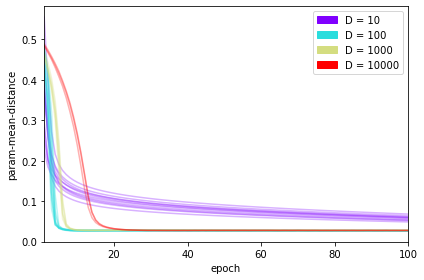
\includegraphics[width=\textwidth]{imgs/conj-pmd-prod-keep50-1t.png}
        \caption{1-term conjunction}
        \label{fig:conjconvkeepn1}
    \end{subfigure}
    \begin{subfigure}[b]{0.30\textwidth}
        \centering
        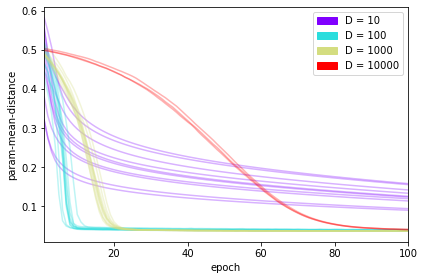
\includegraphics[width=\textwidth]{imgs/conj-pmd-prod-keep50-5t.png}
        \caption{5-term conjunction}
        \label{fig:conjconvkeepn5}
    \end{subfigure}
    \begin{subfigure}[b]{0.30\textwidth}
        \centering
        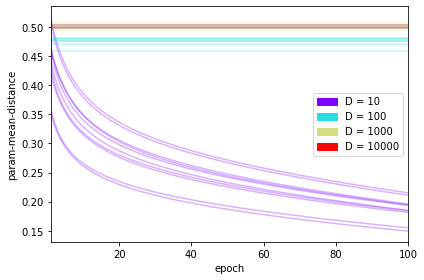
\includegraphics[width=\textwidth]{imgs/conj-pmd-prod-keep50-20t.png}
        \caption{20-term conjunction}
        \label{fig:conjconvkeepn20}
    \end{subfigure}
       \caption{Convergence of mean distance from optimal parameters when learning conjunctions in the Product logic, with the size-50 subset optimisation, under $\XOR$ loss with exponent $a=10$.}
       \label{fig:conjconvkeepn}
\end{figure}

\subsection{Class Imbalance and Parameter Crispness}

In Figure \ref{fig:conjconvkeepn}, we notably see that, whilst applying the subset optimisation makes scaling the dimension of a conjunction viable, what is not viable is increasing the size of the number of terms in the conjunction. If a boolean function is a conjunction of $N$ terms, only a fraction of $2^{-N}$ of all possible inputs will be satisfying. Thus, our learning becomes exponentially worse with increasing $N$. This problem is referred to as class imbalance.

We can explicitly sample the gradients to see how this manifests more directly. Suppose we have a proposed conjunction $\phi(\vx) = x_1 \land x_2 \land x_3$, but we learn that $x_1 = \F$ while $\phi = \T$, for some training data point. If $\phi$ were as we assumed, $\phi$ would be $\F$ in this case, but it is not. Thus $x_1$ cannot be one of the terms in $\phi$. Applying this more generally is what is used in classical algorithms for learning conjunctions given noise-free data \cite{clt}.

We would expect to see a similar effect in the gradient estimator that we derive through backpropagation. To test for this, we uniformly sample random initialisations of a real conjunction model, and observe the gradient estimations that result from an entire epoch of training inputs. Figure \ref{fig:conjgrad1} displays the results of this procedure. A conjunction over $D=10$ variables containing $N=4$ present terms was used to best convey the issue in the empiric results.

\begin{figure}[H]
    \centering
    \begin{subfigure}[b]{0.47\textwidth}
        \centering
        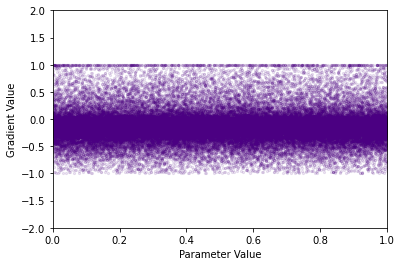
\includegraphics[width=\textwidth]{imgs/grad_prod_1_falseparam.png}
        \caption{Gradient samples for correct parameter $\F$}
        \label{fig:conjgrad1false}
    \end{subfigure}
    \begin{subfigure}[b]{0.47\textwidth}
        \centering
        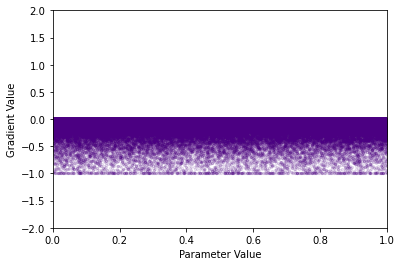
\includegraphics[width=\textwidth]{imgs/grad_prod_1_trueparam.png}
        \caption{Gradient samples for correct parameter $\T$}
        \label{fig:conjgrad1true}
    \end{subfigure}
    \begin{subfigure}[b]{0.47\textwidth}
        \centering
        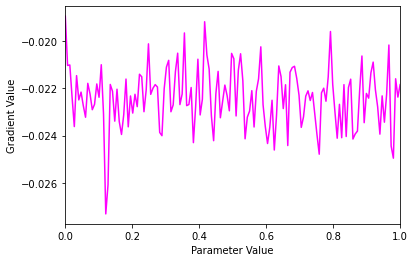
\includegraphics[width=\textwidth]{imgs/grad_prod_1_falseparam_avg.png}
        \caption{Mean gradient estimator for correct parameter $\F$}
        \label{fig:conjgrad1falseavg}
    \end{subfigure}
    \begin{subfigure}[b]{0.47\textwidth}
        \centering
        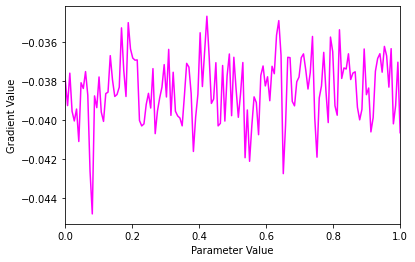
\includegraphics[width=\textwidth]{imgs/grad_prod_1_trueparam_avg.png}
        \caption{Mean gradient estimator for correct parameter $\T$}
        \label{fig:conjgrad1trueavg}
    \end{subfigure}
       \caption{Gradient estimations over the problem of real conjunctions under $\XOR$ loss with exponent $a=1$.}
       \label{fig:conjgrad1}
\end{figure}

We do see that the gradient estimator behaves differently depending on the true valuation of a given logical parameter. If the true value is $\F$, any input sample with a correct output of $\T$ results in a positive gradient estimation, thus decreasing the parameter on the next optimisation step, as can be seen in Figure \ref{fig:conjgrad1false}. This is exactly the kind of behaviour we would expect, and it represents a faithful translation of logical inference to the real domain. Whenever the output is $\F$, the model increases all parameters, as no meaningful inference can be made, which can be seen in both Figures \ref{fig:conjgrad1false} and \ref{fig:conjgrad1true}. This can be interpreted as the model aiming to be robust to noisy data. 

The samples above show that it is impossible for terms which are indeed part of the true conjunction to not be represented in the learnt model, as their parameterisations can only increase. The mean gradient estimator in Figure \ref{fig:conjgrad1trueavg} reflects this, as it is firmly below 0 no matter the parameterisation. If the term is not in the true conjunction, however, Figure \ref{fig:conjgrad1falseavg} shows that we unfortunately see that the gradient estimator is still negative, meaning the term appears in the learnt conjunction, regardless of initial parameterisation. 

This is the result of the class imbalance problem. Despite the gradients being in the right direction at every step, the overall result is inaccurate, because inferences are not being well capitalised if they cannot be frequently made.

What is interesting is that increasing the value of the exponent $a$ appears to resolve this issue. In all our successful tests, we use a value of $a=10$. A plot of gradient samples can be found in Appendix \ref{fig:conjgrad10}. We see that as the exponent increases, the direction of the gradients become more accurate, and the magnitude of the gradients become larger for significantly incorrect values. However, for parameter values that are near to $0.5$, no significant gradient is observed. Values 0 and 1 are referred to as ``crisp'' boolean values, so one could interpret this as the regime failing to ``crispen'' values effectively, despite correctly signed gradients. Appendix \ref{section:moregradients} contains further examples of how this loss fails due to the curse of dimensionality - in all the plots in this section, we use dimensionality $D=10$, but for $D=100$ the gradients quickly vanish.

A significant observation therefore, which was eluded to in the previous section, is that binary cross-entropy, with appropriate choice of logic, suffers none of these problems. 


\begin{figure}[H]
    \centering
    \begin{subfigure}[b]{0.47\textwidth}
        \centering
        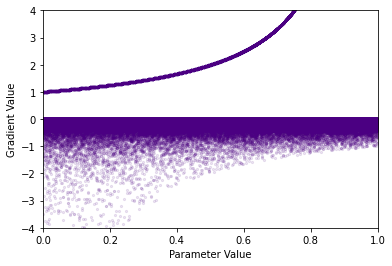
\includegraphics[width=\textwidth]{imgs/grad_prod_bce_falseparam_10dim.png}
        \caption{Gradient samples for correct parameter $\F$}
        \label{fig:conjgrad1falsebce}
    \end{subfigure}
    \begin{subfigure}[b]{0.47\textwidth}
        \centering
        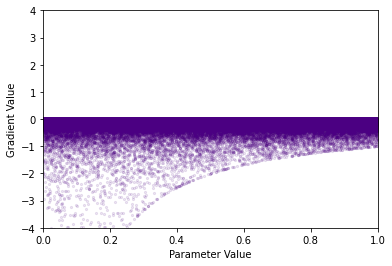
\includegraphics[width=\textwidth]{imgs/grad_prod_bce_trueparam_10dim.png}
        \caption{Gradient samples for correct parameter $\T$}
        \label{fig:conjgrad1truebce}
    \end{subfigure}
    \begin{subfigure}[b]{0.47\textwidth}
        \centering
        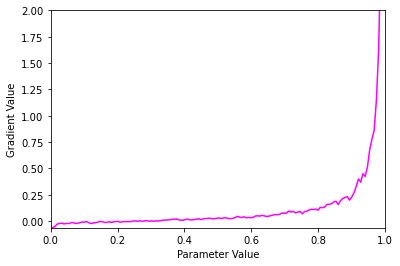
\includegraphics[width=\textwidth]{imgs/grad_prod_bce_falseparam_10dim_avg.png}
        \caption{Mean gradient estimator for correct parameter $\F$}
        \label{fig:conjgrad1falseavgbce}
    \end{subfigure}
    \begin{subfigure}[b]{0.47\textwidth}
        \centering
        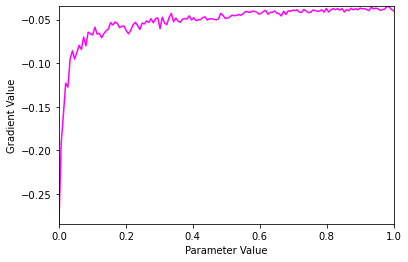
\includegraphics[width=\textwidth]{imgs/grad_prod_bce_trueparam_10dim_avg.png}
        \caption{Mean gradient estimator for correct parameter $\T$}
        \label{fig:conjgrad1trueavgbce}
    \end{subfigure}
       \caption{Gradient estimations over the problem of real conjunctions under binary cross-entropy loss.}
       \label{fig:conjgrad1bce}
\end{figure}

Figure \ref{fig:conjgrad1bce} shows how binary-cross entropy loss not only has a gradient estimator with correct direction, but also of greater magnitude, regardless of current parameterisation. Later empirical results will show that this does have a profound effect on convergence.

We have demonstrated that varying our choice of loss has a significant effect on not only the rate of convergence, but the correctness thereof. Appendix \ref{section:moregradients} contains more such examples, that show how varying the logic, dimension and choice of loss function have an effect on the gradient estimator.

\subsection{Empiric Comparison of Logics}

We have discussed what effect varying the choice of logic has on the gradient estimator $\nabla_\forall$, but we have not seen what effect this directly has on convergence. Figure \ref{fig:conjconvlogics} shows that this effect is profound. Here, a ``correct'' parameter is one which is within $0.5$ of it's optimal value.

\begin{figure}[h]
    \centering
    \begin{subfigure}[t]{0.45\textwidth}
        \centering
        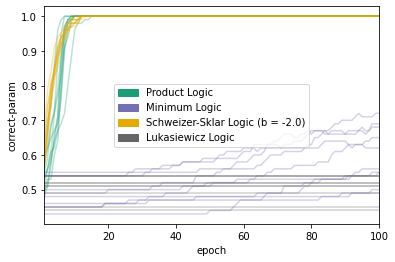
\includegraphics[width=\textwidth]{imgs/conj-cp-100dim-keep50-5t.png}
        \caption{Proportion of correct parameters for $D=100$}
        \label{fig:conjconvcpd100}
    \end{subfigure}
    \begin{subfigure}[t]{0.45\textwidth}
        \centering
        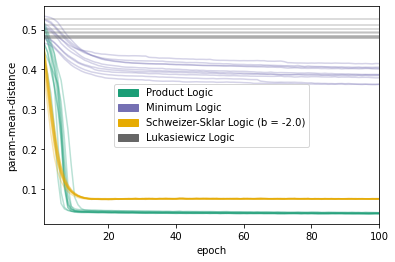
\includegraphics[width=\textwidth]{imgs/conj-pmd-100dim-keep50-5t.png}
        \caption{Mean distance of parameters from optimum for ${D=100}$}
        \label{fig:conjconvpmdd100}
    \end{subfigure}
    \begin{subfigure}[t]{0.45\textwidth}
        \centering
        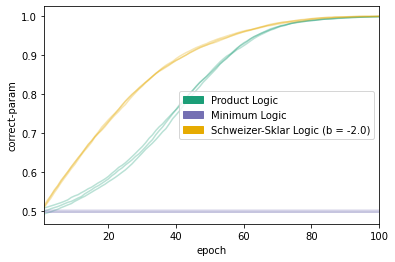
\includegraphics[width=\textwidth]{imgs/conj-cp-10000dim-keep50-5t.png}
        \caption{Proportion of correct parameters for $D=10000$}
        \label{fig:conjconvcpd10000}
    \end{subfigure}
    \begin{subfigure}[t]{0.45\textwidth}
        \centering
        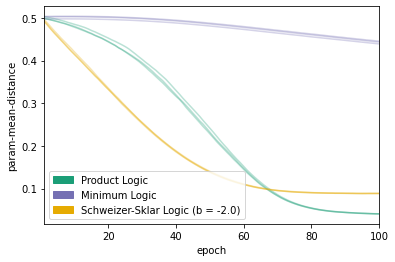
\includegraphics[width=\textwidth]{imgs/conj-pmd-10000dim-keep50-5t.png}
        \caption{Mean distance of parameters from optimum for ${D=10000}$}
        \label{fig:conjconvpmdd10000}
    \end{subfigure}
       \caption{Convergence over various logics under $\XOR$ loss $a=10$, $N=5$ terms, subset optimisation.}
       \label{fig:conjconvlogics}
\end{figure}

\begin{wrapfigure}[12]{r}{0.45\linewidth}
    \centering
    \vspace{-35.0pt}
    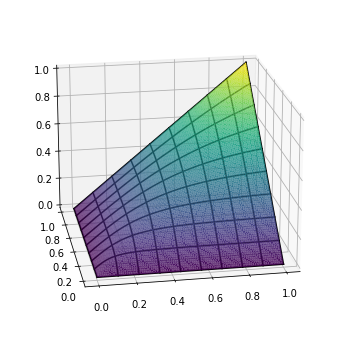
\includegraphics[width=0.30\textwidth, height=0.30\textwidth]{imgs/fuzzy_ss-2_and.png}
    \vspace{-10.0pt}
    \caption[width=0.3\textwidth]{Schweizer-Sklar T-norm ($b=-2$)}
    \label{fig:ssand}
\end{wrapfigure}

The plots show that, as in Figure \ref{fig:toyconv}, Lukasiewicz logic fails even with the discussed optimisations. 

Minimum logic is not far behind - while Figure \ref{fig:conjconvcpd100} shows the proportion of correct parameters increasing gradually for $D=100$, this proportion does not improve whatsoever for $D=10000$. This may be due to the fact that in Minimum logic, only one input variable to a conjunction has non-zero gradient at a time, as can be seen in Figure \ref{fig:minconj}. This restriction does not allow the optimisation regime to traverse the parameter space in an efficient manner. \cite{analyzefuzzy} refers to this problem as the \textit{binarization} of gradients. Empirical examples of this binarization can be found in Appendix \ref{fig:conjgrad10m}.

We have already mentioned in Section \ref{section:prodvanishgradient} that Product logic suffers it's own curse of dimensionality, and we can see this in how it initially has poor convergence in Figure \ref{fig:conjconvcpd10000}. However, as parameters are optimised, the all inputs to the conjunction approach 1, and thus the gradients increase in value. This results in a quickening in convergence rate around 40 epochs, before finally plateauing.

We also see the Schweizer-Sklar logic performs very efficiently, as the bounds derived in Appendix \ref{section:ssbounds} predict. What is interesting to note is that, for $p=0$, Schweizer-Sklar logic is precisely the Product logic, and for $p=-\infty$, it is precisely the Minimum logic. We can therefore also interpret Schweizer-Sklar (with a parameter $p=-2$ as used in the tests) as being a ``middle ground'' between the two logics, having a guaranteed significant gradient without suffering from binarization. 

Of note is that, as we can see in Figure \ref{fig:conjconvpmdd10000}, Product logic still outperforms Schweizer-Sklar logic in the ``crispness'' of it's learnt real parameters, as the former converges to an average distance considerably lower than that of the latter. Under binary cross-entropy loss, we see an interesting result. 

Figure \ref{fig:conjconvlogicsbce} shows the result of training under binary cross-entropy loss, both with and without the subset optimisation. The subset optimisation continues to work with the Product logic, albeit not as well. It however has a disasterous effect on Schweizer-Sklar logic, which not only fails to converge to optimal values, but goes in the wrong direction.

This is not observed without the subset optimisation. As we'd expect, the curse of dimensionality results in the Product logic implementation failing to converge at all. The Schweizer-Sklar implementation performs spectacularly well. It is significantly more efficient than under $\XOR$ loss - under $\XOR$ loss, with a dimensionality $D=10000$, it takes roughly 40 epochs to achieve parameter correctness greater than 90\%. Under binary cross-entropy loss, it only takes around 5. It further improves in the crispness of it's learnt parameters. In Figure \ref{fig:conjconvlogics}, we saw that every logic failed to achieve optimal (i.e. close to 0) distance from optimal parameters. Under this regime, however, we can achieve this. 

\begin{figure}[h]
    \centering
    \begin{subfigure}[t]{0.45\textwidth}
        \centering
        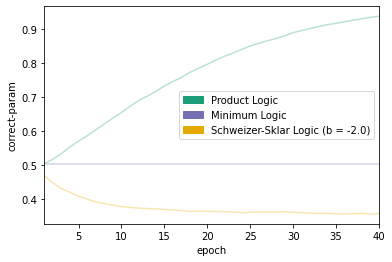
\includegraphics[width=\textwidth]{imgs/conj-cp-10000dim-keep50-5t-bce.png}
        \caption{Proportion of correct parameters with subset optimisation.}
        \label{fig:conjconvcpbceso}
    \end{subfigure}
    \begin{subfigure}[t]{0.45\textwidth}
        \centering
        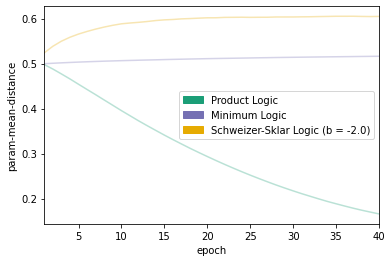
\includegraphics[width=\textwidth]{imgs/conj-pmd-10000dim-keep50-5t-bce.png}
        \caption{Mean distance of parameters from optimum with subset optimisation.}
        \label{fig:conjconvpmdbceso}
    \end{subfigure}
    \begin{subfigure}[t]{0.45\textwidth}
        \centering
        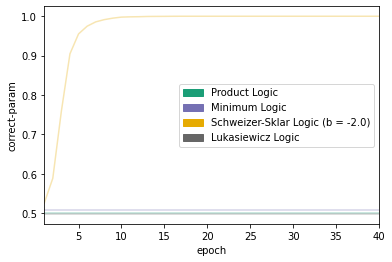
\includegraphics[width=\textwidth]{imgs/conj-cp-10000dim-5t-bce.png}
        \caption{Proportion of correct parameters without subset optimisation.}
        \label{fig:conjconvcpbce}
    \end{subfigure}
    \begin{subfigure}[t]{0.45\textwidth}
        \centering
        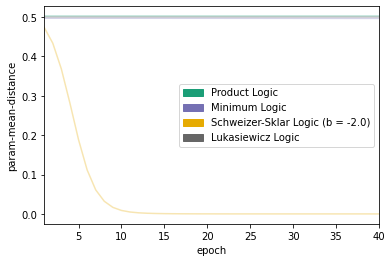
\includegraphics[width=\textwidth]{imgs/conj-pmd-10000dim-5t-bce.png}
        \caption{Mean distance of parameters from optimum without subset optimisation.}
        \label{fig:conjconvpmdbce}
    \end{subfigure}
       \caption{Convergence over various logics under binary cross-entropy loss, $N=5$ terms, $D=10000$ dimensionality.}
       \label{fig:conjconvlogicsbce}
\end{figure}

\subsection{Suboptimal Predictions}

Crispness is important if we wish to use any of these models to actually predict outputs. Suppose that we have correct parameterisations for every term, but with a distance of 0.25 from crisp values $0, 1$. In product logic, $0.25 \limply 0 = 0.75$, whereas in classical logic this would round to $\F \limply \F = \T$. taking the product over a number of such terms that increases linearly with $N$ gives us an upper bound of $O(0.75^N)$ for the actual output. Since randomly sampled input bits generally have a proportion of bits with value $0$ close to $\frac{N}{2}$, most outputs are guaranteed to be near $0$. While many regimes can guarantee 100\% of parameters are ``correct'', the nature of fuzzy logic means the output isn't necessarily translated into correct outputs.

Figure \ref{fig:conjconvco} shows the convergence of the proportion of corrects outputs under various regimes. Of note is that, for $N \geq 100$ under Product logic, the proportion of correct outputs does not meaningfully differ through optimisation. The stagnant proportion is also somewhat around $1 - 2^{-5} \approx 0.968$, which suggests that the output only ever evaluates to false, as this $2^{-5}$ represents the proportion of true outputs for conjunctions of 5 terms. 

This is not surprising, as we have just discussed how this model poorly approximates the true crisp parameterisations $0,1$, which would result in the output degrading to $0$, even if the parameters are all correct.

However, as we have discussed, Schweizer-Sklar logic can approximate crisp values, and does not suffer the curse of dimensionality (as much). This can be observed in Figure \ref{fig:conjconvcoss}. In fact, convergence seems to suffer only linearly in $\log D$.

\begin{figure}[h]
    \centering
    \begin{subfigure}[t]{0.30\textwidth}
        \centering
        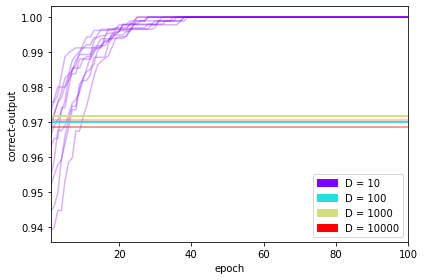
\includegraphics[width=\textwidth]{imgs/conj-co-prod-keep50-5t.png}
        \caption{Product logic, subset optimisation, $\XOR$, $a=10$ loss.}
        \label{fig:conjconvcopxor}
    \end{subfigure}
    \begin{subfigure}[t]{0.30\textwidth}
        \centering
        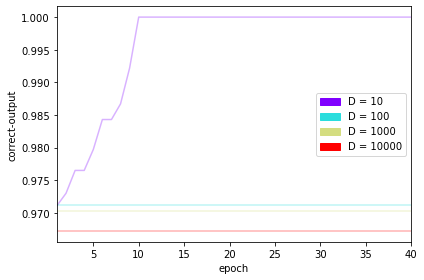
\includegraphics[width=\textwidth]{imgs/conj-co-prod-keep50-5t-bce.png}
        \caption{Product logic, subset optimisation, binary cross-entropy loss.}
        \label{fig:conjconvcopbce}
    \end{subfigure}
    \begin{subfigure}[t]{0.30\textwidth}
        \centering
        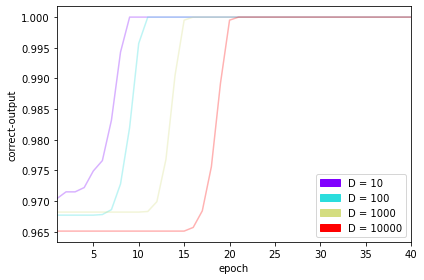
\includegraphics[width=\textwidth]{imgs/conj-co-ss-nokeepn-5t-bce.png}
        \caption{Schweizer-Sklar logic $p=-2$, no subset optimisation, binary cross-entropy loss.}
        \label{fig:conjconvcoss}
    \end{subfigure}
       \caption{Convergence of proportion of correct outputs, $N=5$ terms.}
       \label{fig:conjconvco}
\end{figure}

\subsection{Conclusions}

In learning conjunctions, we have experimented with a variety of logics, loss functions, and additional optimisations to find solutions to the many issues experienced in relaxing classical logic to the real domain. Class imbalance results in inaccurate gradient estimators, while the curse of dimensionality results in vanishing ones. Many logics have gradient estimators which are precisely 0 in a non-negligible region of the parameter space. Even in logics where this isn't the case, for example the Minimum logic, we still suffer due to the gradients being \textit{binarized}, we can only optimise one input at a time. Finally, the lack of crispness in our learnt parameters prevents the predicted outputs from being accurate.

If we learn this problem using Schweizer-Sklar logic under a binary cross-entropy loss, we can resolve all these issues to a satisfactory level. Formal lower bounds exist on the magnitude of the gradient estimator for increasing dimensionality, and class imbalance does not as significantly effect the correctness of the gradient direction under this loss. We can now experiment with more complicated problems. 

\pagebreak

\section{Learning Arbitrary Functions}

An important result from CLT is that with the assumption that $\textsc{RP} \neq \textsc{NP}$, it can be shown that learning boolean functions in DNF is not PAC-efficient \textit{in general} \cite{clt}. Hopefully, relaxing boolean constraints from the discrete to the real domain would allow us to overcome this issue.

\todo{Add test results here}

\todo{Add analysis}

It is important to note that 

- Suddenly not convex (much like MLP)
- Suffers greatly


\section{Alternative Frameworks}

The toy problems above show that the framework we have introduced is not adept at learning boolean functions in general. The appeal instead is that it is simple, and \textit{extensible}. A neurosymbolic layer as we have described can be embedded within a larger model, that may also contain traditional perceptron layers. These mixed models could lend their correctness to traditional NN theory, and their interpretability to their neurosymbolic aspect. In this section, we will discuss other existing neurosymbolic methods, and judge them based on the possibility of use in this application.

One common feature of many of the architectures we have not yet discussed is that logical variables $\vx$ explicitly describe some parent object. In the language of our real logic architecture, there exists some universe of objects $O$ such that boolean inputs to $\phi$ describe an object $o \in O$ in the form of a \textit{unary atom}, e.g. $\textsc{isGreen}(o), \textsc{isBig}(o)$. The output of $\phi$ can be interpreted as the valuation of a further unary predicate. Learning $\phi$ is equivalent to learning some ``if and only if" relationship between different properties of the object $o\in O$, if such a relationship exists. 

\subsection{Alternative Applications of Real Logic}

As mentioned previously, classical symbolic approaches to AI research involve the use of ILP systems. A formal description of an ILP system is one which can solve problems of the following form. Given some background knowledge $B$ of the world of objects $O$ in the form of a logical statement, and new observations of \textit{positive and negative examples} $E^+$ and $E^-$, expressed as conjunctions of \textit{ground literals} (e.g. $\textsc{isGreen}(o), \lnot \textsc{areFriends}(a,b)$), we aim to find some hypothesis statement $h$ such that $B \land h$ satisfies all new observations. Formally, we require \textit{sufficiency} $B \land h \lentails E^+$, and \textit{consistency} $B \land h \land E^- \lnentails \F$ of the constructed $h$.

Our current real logic framework solves a real relaxation of the ILP problem where $E^+$ and $E^-$ are all instances of the same unary predicate. There exist differentiable real logic solvers for general ILP problems \cite{diffilp}, \cite{diffilpGT}. Such implementations improve on classical ILP methods as they are robust to noisy data while still being adept at pattern finding.

Other implementations relax real logic further by removing the requirement for all T-norm axioms to be satisfied. \cite{lnnibm} introduces \textit{Weighted Non-Linear Logic}, which is conceptually similar to Łukasiewicz logic with the addition of a bias parameter $\beta$ which is also optimised during learning. The source paper promotes this reformulation as it removes constraints from the problem of optimisation, though the algorithm introduced in the paper as stated cannot be embedded into a mixed model.

\subsection{Embedded Logic and Relations}

Many developments is neurosymbolic learning involve embedding objects into $n$-dimensional real vector spaces to exploit properties of this space. Word2vec \cite{word2vec} is a model for learning optimal embeddings of natural language atoms in a high-dimensional vector space. Such embeddings were found to preserve relationships between words through vector arithmetic \cite{word2vecrelations} (e.g. Father $-$ Man $+$ Woman $\approx$ Mother). This can be interpreted as a (relaxed) ILP system which learns over the space of \textit{binary} atoms. Learning embeddings of objects $o \in O$ in this manner will aid in extending our current real logic model to mixed models.

In \cite{ltn2016}, the notion of a \textit{grounding} is introduced - before applying any real logic operators, objects $o \in O$ are mapped into $\R^n$ through some canonical function $\calG : O \to \R^n$. An $m$-ary predicate $P$ is then interpreted as a function $\R^{n\times m} \to [0,1]$. The value of $\calG$ may then be learnt in a manner which best evaluates predicates $P$ for elements of the test dataset. 

Further, \cite{embeddedgoogle} suggests that not only should objects be embedded into a real vector space, but that boolean values should be as well. In this system, boolean values are encoded over an $n$-dimensional unit sphere $S_{n-1}$, and logical operators are required to map the encodings of $\T$ and $\F$ appropriately in this space. Introducing new dimensions may aid in improving model quality, without sacrificing interpretability as activations can be collapsed back into ``real logic'' through a similarity metric $\textsc{Sim}:S_{n-1}^2 \to [0,1]$. Cosine similarity (which corresponds to minimum distance travelling along the unit sphere) is generally used. \cite{embeddedlogicreg} improves upon this by also learning core operators $\land, \lor, \lnot$ as DNNs, with correctness ensured through regularisation rather than the architecture itself. This model has been used to develop high quality collaborative filtering algorithms \cite{embeddedcollabreasoning}.

\subsection{Bayesian Models and Probabilistic Logic}

Another approach which could be considered a continuous relaxation of classical logic is in modelling boolean values as distributions over deterministic values $\{\T, \F\}$. Bayesian methods are well studied for this application, with many efficient methods existing for learning the distributions of random variables expressed in terms of a random field. Probabilistic programming languages \cite{gordon2014probabilistic} are able to describe such problems over Bayesian Networks in an highly interpretable manner. Learning probability distributions over the parameter space $\vw$ may prove a more interpretable solution, and further may solve some of the convergence issues seen due to many problems being non-convex. If we interpret real booleans $[0,1]$ as parameters of a Bernoulli distribution over values $\{\T, \F\}$, we can analogize real logic models using the product logic to modelling a random field such that all parameters $\vw$ are independent of each other. In this interpretation, we see that using general Bayesian models increases the expressivity of our model by introducing dependencies between parameters $\vw$. Arbitrary dependencies can be modelled using Normalizing Flows \cite{normalizingflows}.

Bayesian methods are very general, and many approaches exist which are specialised for uses in logic. Bayesian networks are restrictive as they model variable dependencies as a Directed Acyclic Graph (DAG), whereas many dependencies in logic are cyclic (most notably the relation $\iff$). Markov Networks describe dependencies between random variables as edges in a graph, meaning that any two variables that are not adjacent are conditionally independent. These are used to capture logical inferences in the popular Markov Logic Network (MLN) model \cite{markovlogicnetworks}, which corresponds logical atoms to vertices, and formulae to cliques in the graph. Probabilistic Soft Logic \cite{probsoftlogic} further develops on this by introducing a PPL to describe instances of a model similar to MLNs, which can be used to better interpret the results of learning using such methods.



\begin{comment}
\section{A Useful Logical System}

\subsection{Notation}

The notation of linear algebra is very useful in succinctly describing the nature of a classical perceptron model, but within neurosymbolic layers, we do not have this luxury. Further in this paper, we will discuss many different kinds of logical systems, and we will discuss and compare their qualities in learning. To describe our models, it's useful to phrase the layers we construct in a manner similar to linear algebra.

Given a logical system $\B$, we will define a matrix/vector system much like the standard one. A boolean vector of size $n$ is an element of the set $\B^n$, and similarly a boolean matrix of height $a$ and width $b$ is an element of the set $\B^{a \times b}$. Where we now differ is in matrix algebra - in linear algebra, matrix multiplication is defined like so;
$$\mathbf{AB}_{ij} = \sum_{k}\mathbf{A}_{ik}\cdot\mathbf{B}_{kj}$$

We can define boolean matrix multiplication likewise;
$$\mathbf{AB}_{ij} = \bigvee_{k}\mathbf{A}_{ik}\land\mathbf{B}_{kj}$$

This allows us to motivate a meaning for ``dot products" also;
$$\mathbf{a\cdot b} = \mathbf{a}^\text{T}\mathbf{b} = \bigvee_i a_i \land b_i$$

It would be useful to define element-wise operations on vectors/matrices. For any operator $\circ : \B^2 \to \B$, we write $\mathbf{a} \circ \mathbf{b}$ to mean $(\mathbf{a} \circ \mathbf{b})_i = a_i \circ b_i$. If we want to apply an operator with a constant scalar value to every element of a vector, we can write this likewise, $(\mathbf{a} \circ b)_i = a_i \circ b$, etc.

Finally, if an operator $\circ$ is both associative and commutative, we write $^\circ(\mathbf{a})$ to refer to $a_1 \circ a_2 \circ \cdots$.

Using the above two, we can likewise define the ``dot product" by $\mathbf{a \cdot b} ={^\lor}(\mathbf{a \land b})$. We can use a similar notation as syntactic sugar to define matrix multiplication $\mathbf{AB} ={^\lor}(\mathbf{A \land B})$. This notation allows us to use other operators also, for example standard matrix multiplication would be written by ${^+}(\mathbf{A \times B})$. 

\subsection{Boolean Algebras}

While classical perceptron layers heavily rely on linear algebra, neurosymbolic layers cannot. Instead, we must rely on \textit{boolean algebra} to motivate our models. Boolean algebra is fundamentally different to any algebra motivated by classical arithmetic, as we do not have access to the regular operators $+$ or $\times$. Nevertheless, boolean operators behave much like arithmetic ones. A boolean algebra, formally speaking, is a mathematical object $\B$, which contains elements $\T$, $\F$, and for which we have binary operators $\lor$, $\land$, and a unary operator $\neg$, such that the following axioms always hold.

$$
\begin{aligned}
\text{(Associativity)}
&\ (a \lor b) \lor c = a \lor (b \lor c) \\
&\ (a \land b) \land c = a \land (b \land c) \\
\text{(Commutativity)}
&\ a \lor b = b \lor a \\
&\ a \land b = b \land a \\
\text{(Absorption)}
&\ a \lor (a \land b) = a \\
&\ a \land (a \lor b) = a \\
\text{(Identity)}
&\ a \lor \F = a \\
&\ a \land \T = a \\
\text{(Compliments)}
&\ a \lor \neg a = \T \\
&\ a \land \neg a = \F \\
\text{(Distributivity)}
&\ a \lor (b \land c) = (a \lor b) \land (a \lor c) \\
&\ a \land (b \lor c) = (a \land b) \lor (a \land c) \\
\end{aligned}
$$

We can immediately see the similarities to classical arithmetic. In fact, the above construct is a commutative ring, with some extra properties. 

The above system is very intuitive, as it by design can fully motivate a propositional logic. However, we have not motivated our logical system by direct construction, but by necessitating certain behaviours. We therefore need not restrict ourselves to simply the set $\B=\{0,1\}$, we can define $\B$ however we'd like, and exploit the unique characteristics of the $\B$ we have chosen in our learning.

Let's consider an alternative boolean algebra - given a set $S$, let $\B = {\{ U \subseteq S \}}$, that is, the power set of $S$. It is natural to let $\land$ be the intersection of two sets, and $\lor$ the union. We can further say $\T = S$, $\F = \varnothing$, and $\neg:U \mapsto S \setminus U$. One can immediately see that the above axioms follow from basic facts in set theory. This construction is not useful to us, however, as we cannot differentiate over it.

In practice, we'd really like not to stray too far away from classical logic $\B = \{0,1\}$, and simply approximate classical logic with our choice of $\B$. In this way, our goal is not to necessarily to exploit the properties of a boolean algebra once we have them, but to use the axioms of boolean algebras (and derivations thereof) to measure the quality of hypothetical boolean approximations we propose.

\subsection{Measuring Crispness}

To somehow measure how well our model is behaving like a boolean function, it would be useful to construct a distance metric within our space $\B$. The further away from ideal values $\T$, $\F$ we are, or from basic facts true of all boolean algebras, the worse our model may become to intuit as a logical formula.

There exist well understood ways of doing so already. A metric space $X$ is a set endowed with a \textit{distance metric} $d: X^2 \to R$ with the following properties;

$$
\begin{aligned}
\text{(Identity of Indiscernables)}
&\ d(a, b) = 0 \iff a = b \\
\text{(Symmetry)}
&\ d(a, b) = d(b, a) \\
\text{(Triangle Inequality)}
&\ d(a, b) + d(b, c) \leq d(a, c) \\
\end{aligned}
$$

For example, over classical booleans $\B = \{0,1\}$, a valid metric is $d(a,b) = a +_2 b$, where $+_2$ is addition in the finite field $\mathbb{F}_2$. This can also be interpreted as the function $\XOR(a,b) = (\neg a \land b) \lor (a \land \neg b)$. For boolean vectors $\{0,1\}^n$, a valid distance metric would be the \textit{Hamming distance} $d(\mathbf{a,b}) = {^+}(\mathbf{a} +_2 \mathbf{b})$.

For any boolean algebra $\B$, given $d$, we can define a \textit{vagueness metric}
$$v_d(a) = \min\{d(a, \T), d(a, \F)\}$$

In cases where the choice of $d$ is obvious, we will omit the subscript. We refer to values that have low vagueness as being \textit{crisp}.

\section{A General Neurosymbolic Architecture}

We will see particular implementations of LNNs later. Initially, it is important to discuss some general ideas.

As mentioned previously, the UAT shows us that it is possible to model any boolean function within the framework of MLPs, but we want to restrict the architecture of MLPs such that we could begin to interpret the learnt model as a logical formula, while maintaining full expressiveness. It is well known that any boolean function can be represented in Disjunctive Normal Form (DNF). That is, a formula that takes the form;
$$
\begin{aligned}
\phi(x_1, \dots, x_N) =\ &(a_{11} \land a_{12} \land \dots \land a_{1n_1}) \\
\lor\ &(a_{21} \land a_{22} \land \dots \land a_{2n_2}) \\ 
\lor\ &\cdots \\
\lor\ &(a_{m1} \land a_{m2} \land \dots \land a_{mn_m})
\end{aligned}
$$

where the $a_{ij} \in \{x_1, \dots, x_N, \lnot x_1, \dots, \lnot x_N\}$.

This is very convenient, as it means that any architecture we choose to build can learn this highly regular form, instead of some arbitrarily deep tree of logical operators. To transform this into the language of NNs, we want to somehow decompose the above form into a series of ``logical layers". 

There is a natural homomorphism between subsets $W \subseteq \{1, \cdots, N\}$ and disjunctions $D : \{0,1\}^n \to \{0,1\}$. That is, any disjunction $D$ is fully defined by some set $W$, where
$$D_W(\mathbf{x}) = \bigvee_{i\in W} x_i$$.

If we want to learn the disjunction $D$, it is therefore equivalent to learn the membership of the set $S$. Let $\mathbf{w} \in \B^N$, with $w_i = \mathbbm{1}(i \in S) \in \B$. Then we need only learn the value of the vector $\mathbf{w}$. It is important to note that, in the space $\B = \{0,1\}$, we have an equivalent representation

$$
\begin{aligned}
D_W(\mathbf{x}) 
&= \left(\bigvee_{i \in W} x_i\right) \lor \left(\bigvee_{i \not\in W} \F\right) \\
&= \bigvee_{i} x_i \land w_i \\
&= {^\lor}(\mathbf{w \land x}) = \mathbf{w}^T\mathbf{x}
\end{aligned}
$$

To distinguish this understanding of disjunctions with the simple operation $^\lor(\mathbf{x})$, we will refer to these as \textit{weighted disjunctions}.

This definitely justifies the notation introduced in the previous section. A similar procedure gives us a compact representation of conjunctions, though it is not as minimal;

$$
\begin{aligned}
C_W(\mathbf{x}) 
&= \bigwedge_{i \in W} x_i \\
&= \left(\bigwedge_{i \in W} x_i\right) \land \left(\bigwedge_{i \not\in W} \T \right) \\
&= \bigwedge_i \neg w_i \lor x_i \\
&= {^\land}(\mathbf{w} \Rightarrow \mathbf{x})
\end{aligned}
$$

The above notation allows us to represent boolean functions in DNF, as any formula in DNF is a disjunction of \textit{weighted conjunctions} as seen above. We write this like so.

$$F(\mathbf{x; W}) = {^\lor}({^\land}(\mathbf{W \Rightarrow x \concat \neg x}))$$

Here, $@$ is an operator representing vector concatenation.

Suppose we are given feature valuations $x_1, \dots, x_N$, and we are also given whether said features satisfy some set predicate $P(x_1, \dots, x_N)$. To create a functioning ILP system, it is enough to find some logical formula $\phi$ which is consistent with this predicate, meaning that for all inputs $\mathbf{x}$ we have received, $\phi(\mathbf{x}) = P(\mathbf{x})$. The purpose of LNNs is to use backpropagation to find an approximation to such a solution. By nature, NNs are ``forgetful" in that if the distribution and output value of incoming data changes, they are able to modify their parameterisation accordingly. They therefore aren't guaranteed to be consistent with all input data, but this actually becomes a benefit, rather than a hindrance, when we begin to embed LNN systems within classical NN architectures. 

This embedding is important to note, as the aim of the architecture presented in this paper is not to find \textit{correct} concepts, but \textit{useful} ones. We do not necessarily aim to find hypotheses that perfectly represent known concepts, but concepts that when incorporated into our decision making, allow the player of a game to perform effectively. In that sense, we are using LNNs in a way that is similar in construction, but different in intention to ILPs. This is an important distinction to make when comparing this architecture to existing ones in the space of Neurosymbolic ML, which we will discuss later.

\subsection{Interpreting a Neurosymbolic Layer}

We have constructed layers which represent learnable conjunctions and disjunctions, but how do we go about converting this into a human interpretable format? So far we have discussed an architecture which learns any boolean function in DNF, but is this an ideal way of communicating concepts to humans?

Let's consider what a formula in DNF is actually communicating. Each disjunction is naturally going to represent a single concept, and each conjunction within can be interpreted as being instances of said concept. Using the example of Chess, if we want to learn what it means for a bishop to attack a king, we want to iterate over all instances where a bishop is in a directly diagonal position to a king, with no obstruction. Determining each one of these instances can be done with a conjunction (e.g. Bishop on A1, empty spaces in B2, C3, ..., King on E5), and determining whether any of these conjunctions has occurred is handled by the disjunction. 

In this manner, the disjunction is a set of instances of a particular concept, and the conjunctions are the elements of this set.

Is this the best architecture for interpretability? One may consider an architecture with two DNF layers - that is, concepts building on top of further concepts. This can be incredibly useful - suppose we have both a bishop and a knight attacking the king. The presence of both of these concepts, one can imagine, is greater than the sum of it's parts, so it may be useful to consider this a joint concept. We don't necessarily require a second DNF layer to discover this, as we have shown that a single layer is sufficient to fully express all boolean functions, but for the sake of interpretability, it may be advantageous to add this second layer. This is in stark comparison to conventional NNs, where adding layers generally sacrifices interpretability for the sake of expressiveness. This consideration will become important when comparing different implementations of neurosymbolic architectures in practice.

We can now begin to discuss different ways of actually implementing such an architecture.

\section{Fuzzy Logic}

\def\Bf{\B_\text{f}}

An intuitive, and well researched approach to extending the space of valid boolean values is to consider truth to be ``vague", in the sense that something can be ``somewhat" true or ``somewhat" false. To quantify this, we take boolean values in the closed interval $[0,1]$, rather than simply $\{0,1\}$. This approach is known as \textit{fuzzy logic}.  From here, we will denote the traditional boolean algebra by $\B_2$, and fuzzy logic by $\Bf$. 

It is important to note that while this emulates the definition of a probability measure, it is distinctly not. $\mathbb{P}(x) = \frac{1}{2}$ states that $x$ is true with a probability of $\frac{1}{2}$, which can mean either that in $\frac{1}{2}$ of cases, $x$ appears true (the frequentist interpretation), or that we believe that $x$ is true with $\frac{1}{2}$ certainty (the Bayesian interpretation). In fuzzy logic, $x = \frac{1}{2}$ instead states that $x$ is ``half-true", with 100\% certainty. We are only using fuzzy logic to approximate classical, discrete logic, so it is not important to dwell on the philosophical implications of this. Extending the domain of boolean values means that we have to revisit the definitions of simple logical operators $\lnot, \land$ and $\lor$.

\subsection{Fuzzy Operators}

\def\prodand{\custop{\otimes_\times}}
\def\minand{\custop{\otimes_<}}
\def\lukand{\custop{\otimes_\text{L}}}
\def\draand{\custop{\otimes_\text{D}}}

\def\prodor{\custop{\oplus_\times}}
\def\minor{\custop{\oplus_<}}
\def\lukor{\custop{\oplus_\text{L}}}

We will begin with a generalisation for $\land$, as all further definitions follow from this. We want to find a function $\otimes : \Bf^2 \to \Bf$ which has the same value as $\land$ for $\B_2$, and maintains some natural properties of $\land$ also. Suppose we assume the following axioms for $\otimes$;
$$
\begin{aligned}
\text{(Associativity)}&\ (a \otimes b) \otimes c = a \otimes (b \otimes c) \\
\text{(Commutativity)}&\ a \otimes b = b \otimes a \\
\text{(Monotonicity)}&\ a \leq b, c \leq d \implies a \otimes c \leq b \otimes d \\
\text{(Identity)}&\ \forall a, a \otimes 1 = a
\end{aligned}
$$
 
The axioms are actually already enough to ensure that $\otimes |_{\B_2} = \land$. However, they are not enough to ensure $\otimes$ takes one particular value in the set $\B_\text{f}^2 \to \B_\text{f}$, in fact there are an infinite family of possible functions $\otimes$. The above axioms are known as the \textit{t-norm axioms}, and the functions which satisfy it are known as \textit{t-norms}. Some examples of t-norms are;
$$
\begin{aligned}
    \text{(Product t-norm)}&\ a \prodand b \coloneqq ab \\
    \text{(Minimum t-norm)}&\ a \minand b \coloneqq \min\{a,b\} \\
    \text{(Łukasiewicz t-norm)}&\ a \lukand b \coloneqq \max\{a+b-1,0\}
\end{aligned}
$$

If we can generalise either $\lnot$ or $\lor$, then we can generalise both. A seemingly obvious way to generalise $\lnot$ is by simply declaring that $\lnot x = (1 - x)$. This immediately satisfies the definition of $\lnot$ in classical logic, and comes with some useful properties;
$$
\begin{aligned}
\text{(Self-Invertibility)}&\ \lnot(\lnot a) = a \\
\text{(Monotonicity)}&\ a \leq b \implies \lnot a \geq \lnot b \\
\end{aligned}
$$

From this, we can fully define generalisations for $\lor$, which we call \textit{t-conorms}. In classical logic, we can appeal to \textit{De Morgan's laws}, in that $a \lor b = \lnot (\lnot a \land \lnot b)$. Similarly, we can say that $a \oplus b = \lnot(\lnot a \otimes \lnot b) = 1 - (1 - a) \otimes (1 - b)$, given a particular choice of t-norm $\otimes$. We therefore have;

$$
\begin{aligned}
    \text{(Product t-conorm)}\ a \prodor b \coloneqq &\ 1 - (1-a)(1-b) \\
    = &\ a + b - ab \\
    \text{(Minimum t-conorm)}\ a \minor b \coloneqq &\ 1 - \min\{1-a,1-b\} \\
    = &\ \max\{a, b\} \\
    \text{(Łukasiewicz t-conorm)}\ a \lukor b \coloneqq &\ 1 - \max\{(1-a)+(1-b)-1,0\} \\
    = &\ \min\{a+b, 1\}
\end{aligned}
$$

Given the t-norm axioms, we immediately have some convenient properties of t-conorms also.

$$
\begin{aligned}
\text{(Associativity)}&\ (a \oplus b) \oplus c = a \oplus (b \oplus c) \\
\text{(Commutativity)}&\ a \oplus b = b \oplus a \\
\text{(Monotonicity)}&\ a \leq b, c \leq d \implies a \oplus c \leq b \oplus d \\
\text{(Identity)}&\ \forall a, a \oplus 0 = a
\end{aligned}
$$

The only difference here being that the identity has value 0, rather than 1. From this, we can define every logical formula using fuzzy logic operators, allowing us to motivate an architecture for a fuzzy NN.

In the field of fuzzy logic, the above method of constructing fuzzy operators is not actually the preferred way of doing so. Fuzzy logicians instead choose to define the \textit{residuum} $\Rightarrow$ in terms of fuzzy conjunction $\otimes$. The residuum, as the symbol suggests, is meant to generalise the implication operator $(a \Rightarrow b) = \lnot(a \land \lnot b)$. The reason this can be done only relying on the existence of the t-norm (rather than t-norm + fuzzy negation) is because it can be proven that the residuum is the \textit{only} function that satisfies the conditions
$$a \otimes b \leq c \iff a \leq (b \Rightarrow c)$$

The justification for this fact comes from the understanding of fuzzy logic as measuring ``confidence" - if we have confidence valuations for $a, a \Rightarrow b \in \B_f$, and we know that $a, a \Rightarrow b$ entails $b$ in classical logic, then we would expect to be at least $a \otimes (a \Rightarrow b)$ confident in $b$, i.e. that $a \otimes (a \Rightarrow b) \leq b$. A similar construction results in the conclusion above, and allows us to uniquely determine $\Rightarrow$. From here, we can choose to define the other logical operators like so;

$$
\begin{aligned}
\lnot a =&\ (a \Rightarrow 0) \\
a \oplus b =&\ (\lnot a \Rightarrow b)
\end{aligned}
$$

Again, we will not dwell on this, as we are aiming to construct fuzzy operators specifically to approximate classical logical formulae in DNF. The definitions for negation, conjunction and disjunction given above are more than enough to begin doing so. In the notation introduced previously, we could write a formula for a fuzzy DNF layer like so.
$$
F(\mathbf{x, W}) = {^\oplus}({^\otimes}(\mathbf{W \Rightarrow x \concat \neg x}))$$

\subsection{Constructing Fuzzy Operators}

So far we have declared the existance of operators satisfying the given axioms, but we have not discussed how we might discover new ones. It is important to be able to do so freely, as the convergence rate of an algorithm may have a strong relation to the gradient of the chosen operator. To give an example, an operator known as the \textit{drastic t-norm} is 0 anywhere it doesn't have to be anything else, i.e.
$$a \draand b = \begin{cases}
    a &\text{if } b = 1 \\
    b &\text{if } a = 1 \\
    0 &\text{otherwise}
\end{cases}$$

The gradient of $\draand$ is 0 almost everywhere, which isn't terribly ideal for gradient descent. We want to be able to avoid cases like this, and to do so it would beneficial to come up with a method to construct t-norms reliably. Suppose we had a decreasing function $f:\Bf \to [0,\infty]$ with $f(1)=0$. Then the function $T(a,b) = f^{-1}(\min\{f(0), f(a) + f(b)\})$ is a t-norm - in fact, most common t-norms can be constructed in this way. This statement omits some details, but for our use cases this is fine.

A function $f$ which begets a t-norm in this manner is called an \textit{additive generator} of the t-norm. Some examples are;

$$
\begin{aligned}
\text{(Product t-norm)} &\ f(x) = -\log(x) \\
\text{(Łukasiewicz t-norm)} &\ f(x) = 1 - x \\
\text{(Drastic t-norm)} &\ f(x) = 2 - x \text{ for } x \in [0,1), f(1) = 0\\
\end{aligned}
$$

This characterisation of t-norms also allows us to explicitly define conjunctions over many variables - if $a \otimes b = f^{-1}(\min\{f(0), f(a) + f(b)\})$, then ${^\otimes}(\mathbf{x}) = f^{-1}(\min\{f(0),{^+}(f(\mathbf{x}))\})$. Thus,

$$
\begin{aligned}
^\prodand(\mathbf{x}) &= {^\times}(\mathbf{x}) \\
^\lukand(\mathbf{x}) &= \max\{0, 1 + {^+}(\mathbf{x} - 1)\}
\end{aligned}
$$


and so on. In the construction of t-norms from additive generators, we have to add a $\min$ operation, as the sum $f(a) + f(b)$ may be out of the range of $f$. If there exist $a,b \neq 0$ such that this is the case, we refer to the corresponding t-norm as \textit{nilpotent}, since $a \otimes b = 0$. More accurately, this name arises due to the fact that for such $a \neq 0$, there exists $n \in \N$ such that $\underbrace{a \otimes \cdots \otimes a}_{n \text{ times}} = 0$. 

Examples of nilpotent t-norms are the Łukasiewicz t-norm $\lukand$, and the drastic t-norm $\draand$. In fact, any t-norm whose additive generator is continuous around $0$, and doesnt cover the full possible range $[0, \infty]$, is nilpotent in this manner. Any nilpotent t-norm has a non-negligible region of zero gradient, so this will help inform our future discussion on constructed t-norms.

\subsection{Defuzzification and Interpretation}

Suppose we have embedded a fuzzy LNN layer into our larger neural network. How do we go about interpreting the parameterisation of the function? We have already discussed how we may approach doing so for classical DNFs, but to achieve anything at all, we would need to be able to do so for fuzzy DNFs as well.

We can avoid this issue by ensuring that we learn parameters that are as close to $\B_2$ as possible. To do so, we may consider applying some regularisation term to our loss function, which negatively weights parameter values that are not very crisp. We could then add a regularisation term $\lambda \sum_w v(w)$ over all parameters $w$, and use cross-validation to find an optimal $\lambda$ for learning.

In practice, this hinders learning quite a bit. Much of the strength of fuzzy logic architectures are a direct result of maintaining vagueness - if we are close to values $0$, $1$, it can take a lot of data to modify this.

A more effective approach in practice seems much more naive - that is to simply clamp the value of the parameters $w$ into the range $[0,1]$ at every optimisation step. This allows the model to maintain a level of vagueness where it cannot learn much information, i.e. not ``jumping to conclusions". When it actually can decide the nature of a concept, it can freely do so. We may then choose to terminate our learning when the parameters are sufficiently close to values $\{0,1\}$.

In future sections, we see that using the distance metric $d$ \textit{can} be quite effective in regularisation, but not for directly ensuring crispness - we will use the function $v$ to evaluate the interpretability of our chosen models, but we will not actively optimise for interpretability, we want the models to passively approach crisp parameterisations.

\section{Parameterised Logic}

So far, we have discussed learning the membership of conjunctions and disjunctions only, while keeping the actual definitions of operators constant. We have discussed the fact that some choices of operators may be more successful in learning through backpropagation than others, with the case of the drastic t-norm $\draand$ being a particularly bad choice. How may we find the \textit{most successful} one? 

It's difficult to quantify what this means, so we will not attempt to do so. Instead, we can find some way of defining parameterised \textit{families} of logical systems, and learn the optimals parameters of these families in the same way we learn the parameters of the formulae we are trying to learn.

\subsection{Parameterised T-Norms}

In the previous section, we discussed an easy way to construct new t-norms, so it would make sense to use this technique here. We would like to find a family of t-norms that are all parameterisations of a more general construction. We can begin by parameterising additive generators, and constructing their respective t-norms likewise.

Let $f_p(x) = \frac{1 - x^p}{p}$. This satisfies all the criteria for an additive generator, since $f_p'(x) = -x^{p-1} \leq 0$, and $f_p(1) = 0$. For $p=0$, this is not well defined, but taking the limit as $p$ approaches 0 allows us to extend the function further. In fact this limit is well known - we can say that $f_0(x)=-\log x$, which is actually the additive generator for the product t-norm $\prodand$. What is the resultant t-norm in general?

Since $f^{-1}_p(x) = (1-px)^\frac{1}{p}$, we have $a \otimes_p b = \max\{0, (x^p + y^p - 1)^\frac{1}{p}\}$, and more generally, ${^{\otimes_p}}(\mathbf{x}) = \max\{0, (1 - {^+}((1 - \mathbf{x})^p))^\frac{1}{p}\}$. Of note is that, for $p=1$, this is the Łukasiewicz t-norm $\lukand$. It seems as though many t-norms we have already encountered are members of this family. Indeed, if we further extend the definition we have to $-\infty, \infty$ via continuity, we discover that $\otimes_{-\infty}$ is the minimum t-norm, and $\otimes_\infty$ is the drastic t-norm.

This is wonderful news, as it means with one parametric family of t-norms, we can capture all the examples we might like to study, and then some. These operators are known as the \textit{Schweizer–Sklar t-norms}. Some more parameterised families of t-norms are given by the following additive generators;

$$
\begin{aligned}
\text{(Yager t-norms)}&\ f(x) = (1-x)^p \\
\text{(Aczél–Alsina t-norms)}&\ f(x) = (- \log x)^p \\
\text{(Hamacher t-norms)}&\ f(x) = \log\frac{p+(1-p)x}{x}
\end{aligned}
$$

\subsection{Biased Logic}

There are many properties of classical logical operators that cannot necessarily be captured by fuzzy operators. \textit{Idempotence} is a resultant property of both $\land$ and $\lor$ in boolean algebras, which specifies that for all $a, b \in \B_2$, $(a \land b) \land b = (a \land b)$, and likewise for $\lor$. For most t-norms, this is specifically not the case - an obvious example is the product t-norm, where $abb=ab \iff b = 1$. It would be nice to preserve idempotence, but this is not really required. What if we can sacrifice other properties of boolean operators as well?

We will introduce a new parameterised family of boolean operators, called \textit{weighted non-linear logic} (WNL). WNL is a generalisation of Łukasiewicz logic which introduces a bias term $\beta$, which mirrors the bias used in perceptron layers of classical NN architectures. 

We will define conjunctions and disjunctions like so 



\subsection{Boolean Regularisation}

\subsection{Measuring Similarity}

\section{General Boolean Embeddings}

So far we have met Fuzzy Logic, which fundamentally reinvents the common perceptron architecture seen in most NNs. What if we want to maintain an architecture which is more conventional in it's approach, while still allowing for boolean interpretations? This seems difficult at first - although we can approximate any boolean function, determining the nature of this function is difficult in conventional architectures, as we have seen.

Rather than modifying the architecture of the network, we can instead regularise an existing network architecture to act like a boolean function, while making sure that the regularisation somehow allows us to easily interpret the network's parameters. This sounds rather involved - how might we begin to approach this?

\subsection{Booleans as Vectors}

We have discussed the idea of embedding values representing $\T$ and $\F$ into a continuous space $\B$, and then differentiating over the space in backpropagation. In fuzzy logic, we specifically fix the set $\B_\text{f}\coloneqq[0,1]$ to act as our continuous space, and exploit this by using continuous functions which are guaranteed to behave like logical operators. What if we instead allow for the full range of parameters $\R$, how may we begin to interpret this as a boolean function?

We can take inspiration from other architectures where feature embeddings are common. In natural language processing, word embeddings are maps which take words in a dictionary, and map them into a finite-dimensional vector space. The position the word is mapped to in this vector space can be used to characterise the meaning of the word, and capture relations between words. We could likewise map the boolean values $\T$, $\F$ into a vector space $\B$, and measure the ``crispness" of a learnt function by how similar certain values are to the boolean embeddings in this vector space.

We can define some sort of ``distance metric" over $\B$, a convex, commutative function $d : \B^2 \to \R$ such that $d(\mathbf{a, a}) = 0$ for all $\mathbf{a} \in \B$. This can be a formal distance metric in the topological sense, but it need not be. With this, we can say that the more distant a value $\mathbf{x} \in \B$ is from both $\T$ and $\F$, the less crisp. A particular example which is effective in practice is given later in this section.

\subsection{Learning a Boolean Operator}

Suppose we want to learn the function $\XOR(a, b) = (a \land \lnot b) \lor (\lnot a \land b)$. The model we will use to approximate this will be a NN with a single hidden layer, as it is well known that this cannot be done by a simple single-layer perceptron model. The model will therefore map values between three spaces, which we will call $\B^2 \to X \to \B$, for some $\B, X$, which we will not yet specify.

From here, we can proceed as usual and simply backpropagate with correct input-output pairs to learn an appropriate parameterisation for $\XOR$. However, we can somewhat cheat, because we know the appropriate behaviours of the function we're trying to learn, we only want to learn it over our arbitrary boolean embedding $\B$. We can exploit known properties of $\XOR$ to ``push along" our learning. For instance, we know that;

$$
\begin{aligned}
\text{(Associativity)}&\ \XOR(\XOR(\mathbf{a, b}), \mathbf{c}) = \XOR(\mathbf{a}, \XOR(\mathbf{b, c})) \\
\text{(Commutativity)}&\ \XOR(\mathbf{a, b}) = \XOR(\mathbf{b, a}) \\
\text{(Identity)}&\ \forall \mathbf{a} \in \B, \XOR(\mathbf{a}, \F) = \mathbf{a} \\
\text{(Negation)}&\ \forall \mathbf{a} \in \B, \XOR(\mathbf{a}, \T) = \lnot \mathbf{a}
\end{aligned}
$$

The meaning of $\lnot\mathbf{a}$ here will be explained the next section. We will define a ``$\XOR$-iness loss",
$$\ell_\XOR(\mathbf{x,y}) = d(\XOR(\mathbf{x, y}),\XOR(\mathbf{y, x})) + d(\XOR(\mathbf{x}, \F), \mathbf{x}) + d(\XOR(\mathbf{x}, \T), \lnot \mathbf{x})$$

We can see that a perfect parameterisation of $\XOR$ would minimise this loss. Thus, a complete loss function would look like so,
$$\ell(\mathbf{x,y,z}) = d(\XOR(\mathbf{x,y}),\mathbf{z}) + \lambda_\XOR \ell_\XOR(\mathbf{x,y})$$

The parameters of $\XOR$ are hidden in this representation, as they need not be of any particular architecture.

\subsection{Measuring Similarity}
 
\section{Overview of Different Architectures}
\end{comment} 
\chapter{LNNs in Practice} 

\chapter{A Chess Architecture}

\chapter{Interpreting Chess}

\chapter{Conclusions}
 
\begin{thebibliography}{1}
\bibitem {gradientattribute}
\href{run:https://link.springer.com/chapter/10.1007/978-3-030-28954-6_9}{Ancona M., Ceolini E., Öztireli C., Gross M. (2019) Gradient-Based Attribution Methods. \emph{Explainable AI: Interpreting, Explaining and Visualizing Deep Learning.} Lecture Notes in Computer Science, vol 11700. Springer, Cham. https://doi.org/10.1007/978-3-030-28954-6\_9}

\bibitem {neuraladditive}
\href{run:https://link.springer.com/chapter/10.1007/978-3-030-28954-6_9}{R. Agarwal, L. Melnick, N. Frosst, X. Zhang, B. Lengerich, R. Caruana, G. Hinton. Neural Additive Models:
Interpretable Machine Learning with Neural Nets. arXiv:2004.13912}

\bibitem {xnn}
\href{run:https://link.springer.com/chapter/10.1007/978-3-030-28954-6_9}{J. Vaughan, A. Sudjianto, E. Brahimi, J. Chen, V. Nair. Explainable Neural Networks based on Additive Index Models. arXiv:1806.01933}

%\bibitem{IEEEhowto:kopka}
%H.~Kopka and P.~W. Daly, \emph{A Guide to {\LaTeX}}, 3rd~ed.\hskip 1em plus
% 0.5em minus 0.4em\relax Harlow, England: Addison-Wesley, 1999.

%\bibitem{lamport} L. Lamport, \emph{ {\LaTeX} A Document Preparation
%  System}, Reading, Mass: Addison-Wesley, 1994.

%\bibitem{knuth} D. E. Knuth, \emph {The \TeX book}, Reading, Mass.:
%  Addison-Wesley, 1996.

\end{thebibliography}
\end{document}